%!TEX root = ../thesis.tex

\section{Blue face subdivision}
\label{s:subdiv}


At this point we have a vertically one-sided graph (due to Lemma \ref{lm:topfan:oneSidedREL}) without large topfans except possibly for the locations provided in Lemma \ref{lm:topfan:remainingTopfans}.

\paragraph{Outline}
In this stage we are going to recolor edges in all blue faces to make all of them $d+1$-sided. We will start at the bottommost face in the creation order (which we will have to recalculate after the topfanflips, but every REL has one). And we will recolor some if it's edges if a blue face that is to large will appear. \fxnote{I may need to expand a bit more on this order}

We then mark the edges on the top boundary path of this face above the recolored edges as \emph{loaded}. This means that we will try to not flip above these edges in future iterations of the algorithm.

Then we continue with the next face in the order we just calculated.


\paragraph{Loads}
\fxwarning{Still have to describe loads}
What is a load, putting trough loads


\paragraph{Step requirements}
We flip edges in each face, taking into account loads on the bottom fence. Such that

\begin{enumerate}
  \item We never load the edge next to a split/merge
  \item We never load two adjacent edges
\end{enumerate}

It's important to note that we put trough edge loads on splits and merges

Because we do this we can also say the following

\begin{lemma}
  \label{lm:}
  On the bottom boundary path of every face we never find two subsequent loaded edges. Even when we put trough loads on splits and merges.
\end{lemma}
\begin{proof}
  A single face would never load two subsequent edges. Hence the only way to get two subsequent loaded edges is using different faces and thus splits and merges.

  However due to the built-in safety of never flipping next to a split/merge we never get subsequent loaded edges.
  \fxnote{Might add a figure}
\end{proof}


\subsection{Faces without large topfans in the midlle}
Let us first consider the base case: no failed top fan flips and thus all topfans are of size exactly $2$.

\begin{lemma}
  \label{lm:subdiv:withoutTopfan}
  We can subdivide any blue face without large topfans into 5-sided chunks while obeying the load rules above.
\end{lemma}

\begin{proof}
  A worst case example is given in Figure \ref{fig:subdiv:worstCase}.

  \begin{figure}[h]
    \centering
    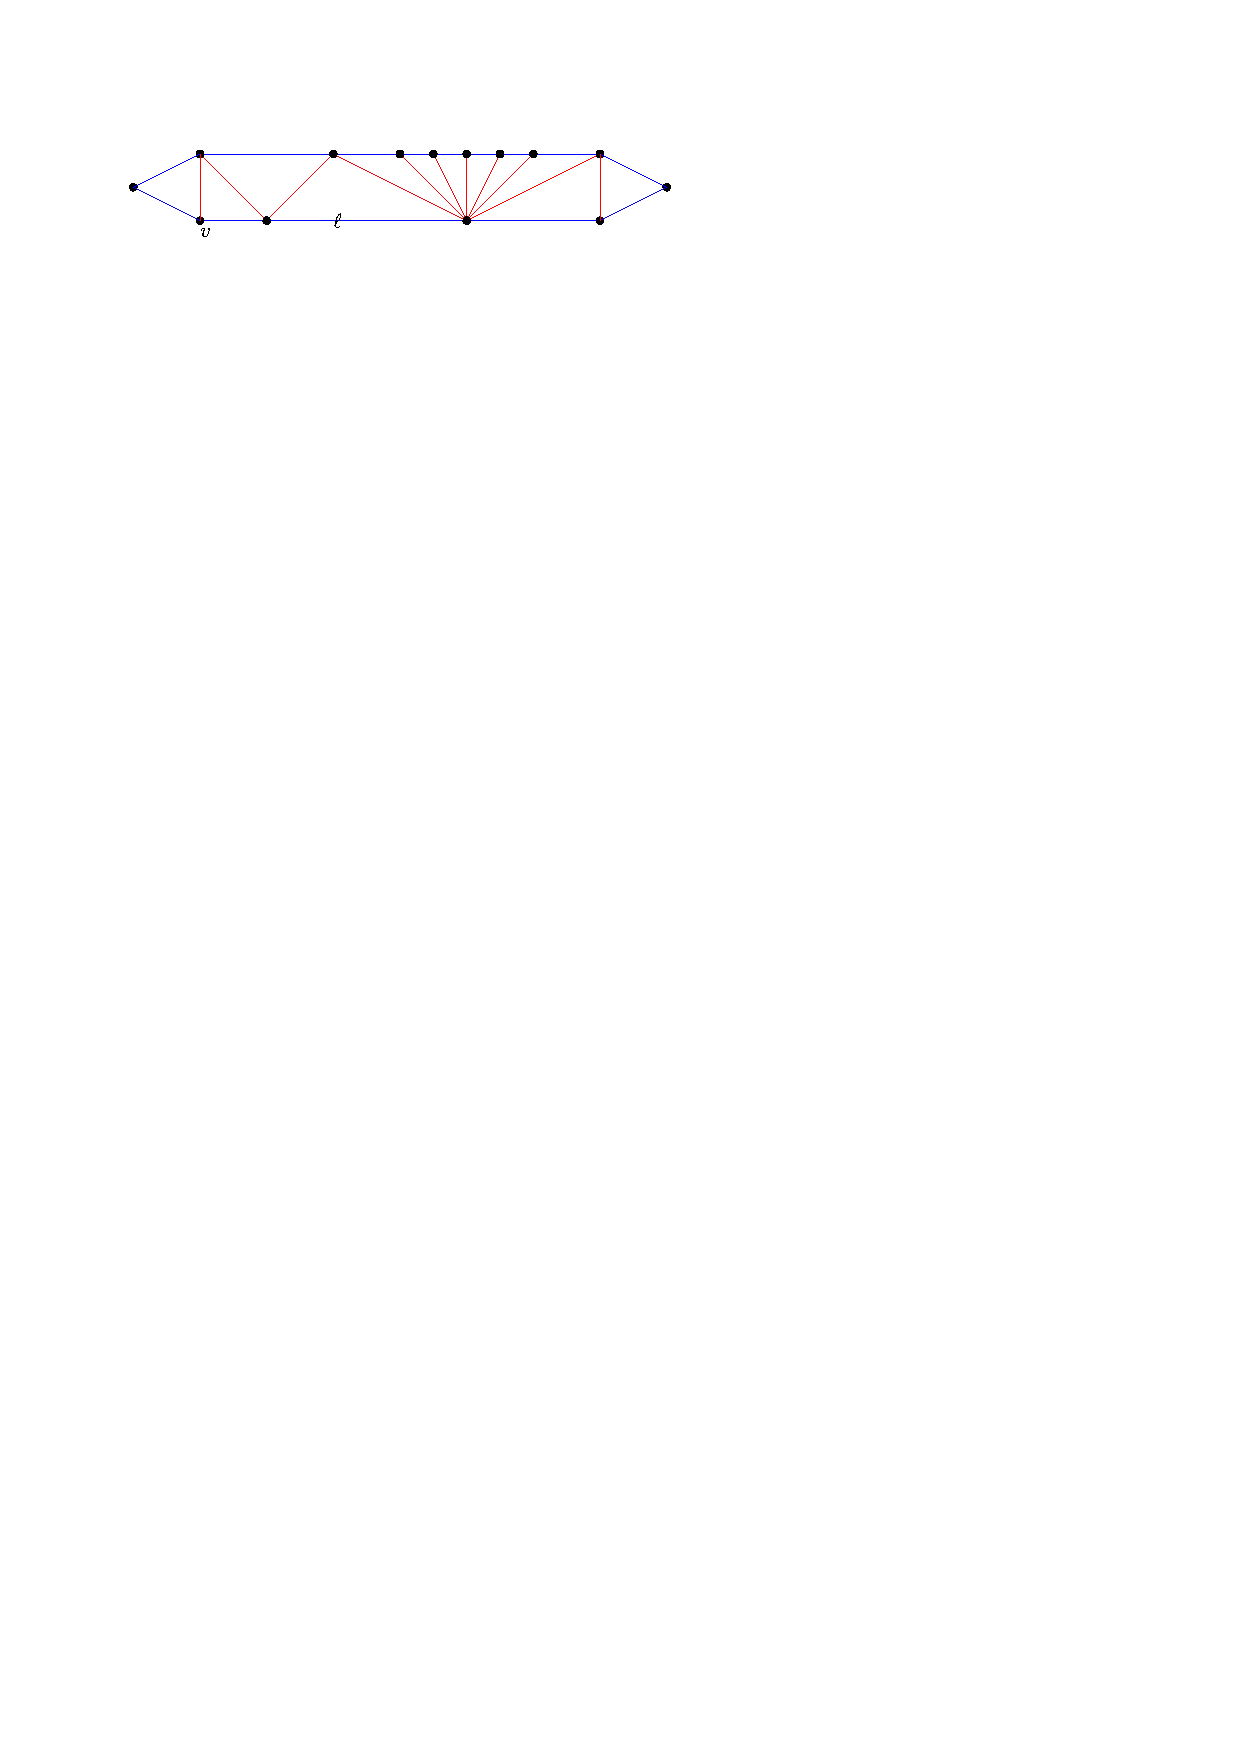
\includegraphics[scale=1]{blueFaceSubdivision/img/worstCase}
    \caption{A worst case blue face. We don't flip any edge in this face.}
    \label{fig:subdiv:worstCase}
  \end{figure}

  Note that we can flip to the right above each edge in the bottom boundary path.

  We will look at the vertex on the bottom fence that's adjacent to the freshly flipped edge, or if we haven't flipped an edge yet the vertex next to the split (and we will call it $v$). The following are then the rules for flipping above the edges following $v$.
  \begin{enumerate}
    \item We don't flip above the first edge.
    \item We flip above the second edge if it's unloaded.
    \item Otherwise we flip above the third edge.
    \item We never flip next to the merge the merge
  \end{enumerate}

  When flipping above a edge we always flip the right edge above that edge.

  The first edge give us the required separation of loaded edges along the top boundary path. The other items make sure we obey the other rules in a straightforward manner.

  The worst case is given by a combination of the last two items. We would in that case want to flip above the third edge. But we don't because the next edge is the merge. This gives at worst 5 edges along the whole bottom boundary path and hence a 4-sided face.



\end{proof}

See Figure \ref{fig:subdiv:sampleExecution} for a sample execution of the algorithm described in Lemma \ref{lm:subdiv:withoutTopfan}.

\begin{figure}[h]
  \centering
  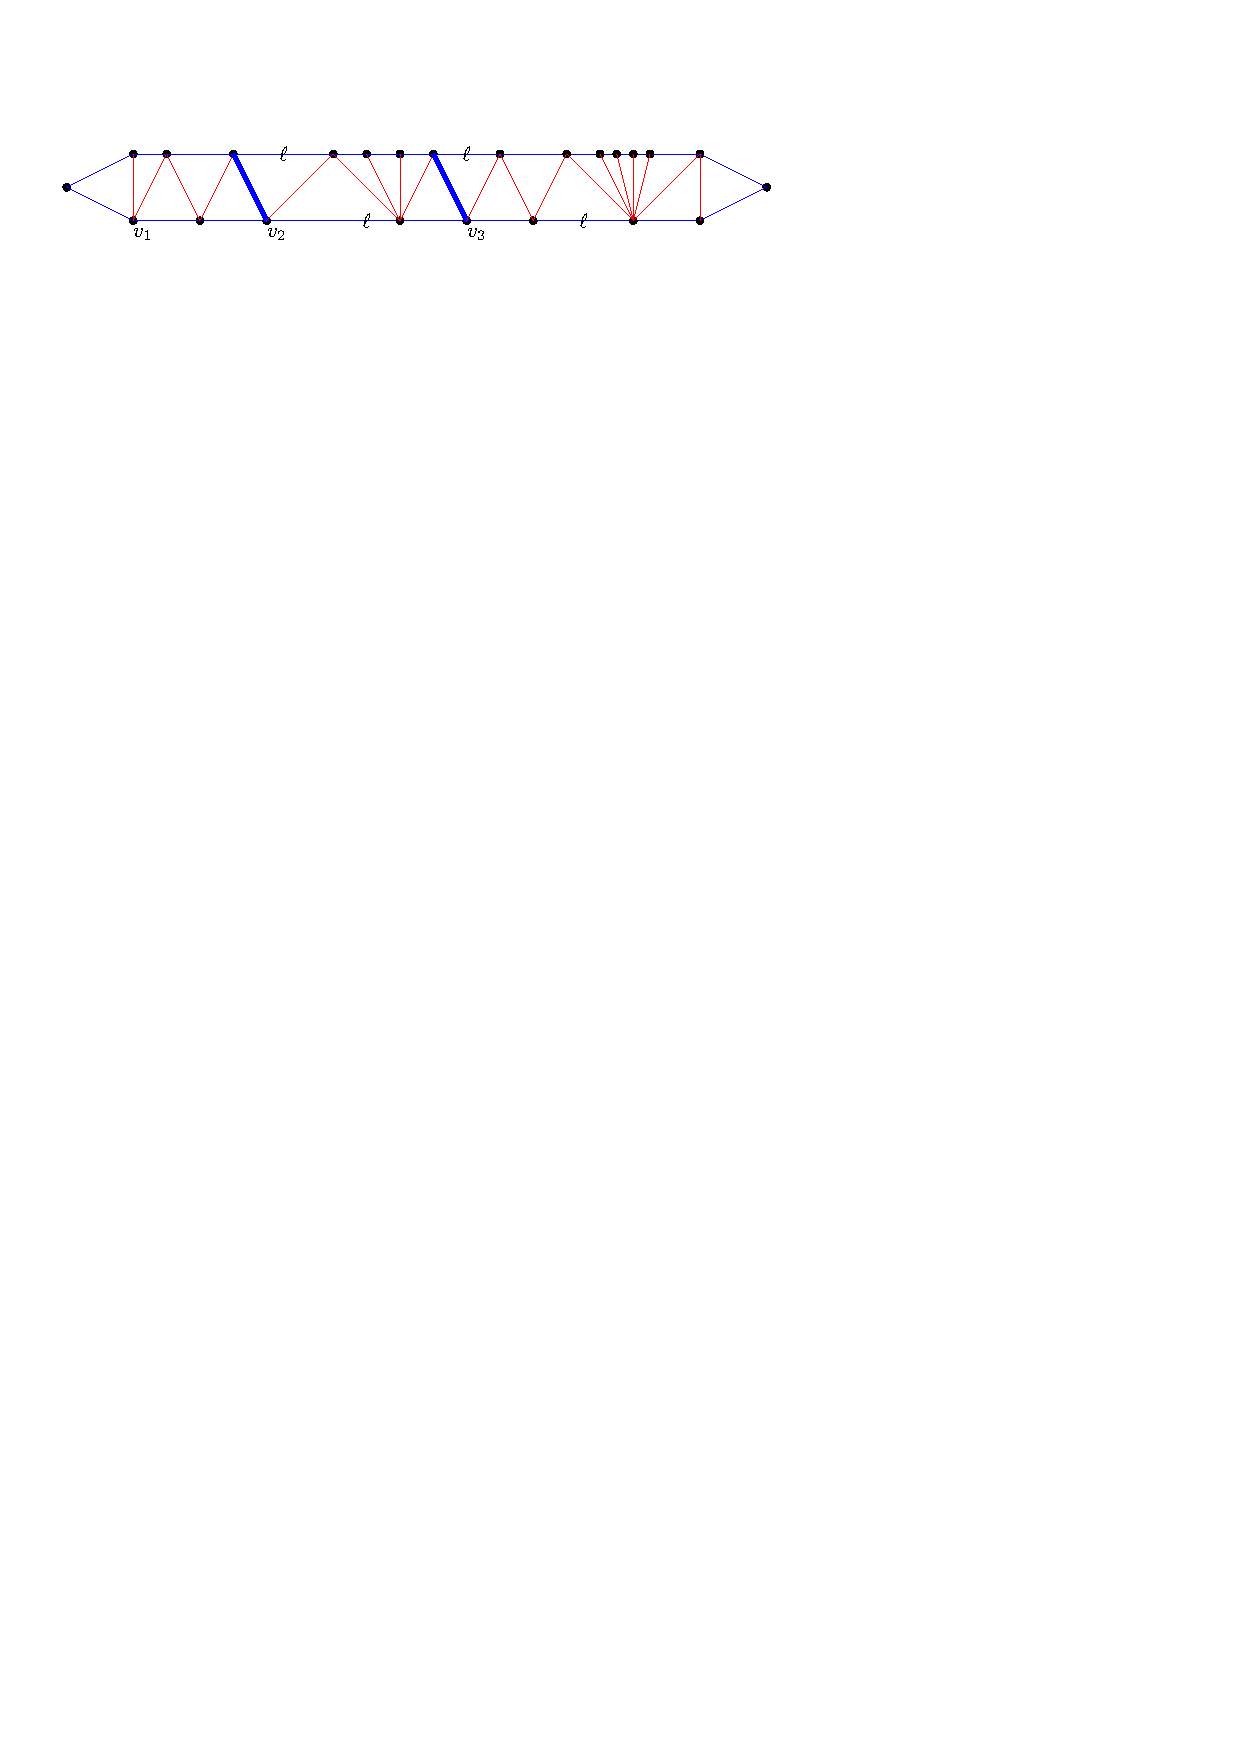
\includegraphics[scale=1]{blueFaceSubdivision/img/sampleExecution}
  \caption{Sample execution of the algorithm}
  \label{fig:subdiv:sampleExecution}
\end{figure}


\subsection{Face starting with a large topfan}
The same algorithm as in Lemma \ref{lm:subdiv:withoutTopfan} after skipping the first topfan instead of the first edge finds us a finds us an edge keeping this face as a $ d - 3 +3 = d$ face.
\fxnote{Might add figure of worst case.}

\subsection{Face encountering a larger topfan}
If we have a large topfan in the middle of the face then above the left outer edge of this topfan we can't have another topfan that failed to flip its left outer edges by Lemma \ref{lm:sweep:NoTwoSplitsAboveEachOther}.

This means we can use the following rule: we flip the first edge of a topfan even above a loaded edge. And still make only chains of at most $2$ $Z$'s.


\subsection{General conclusion}
\begin{lemma}
  \label{lm:subdiv:2chaindedZ}
  Two chained $Z$'s give at worst a $d-1$-sided face
\end{lemma}
\begin{proof}
  Before creating the $Z$'s in this section the \rel was vertically onesided. This also implies that  any $Z$ we now create can have at most one large merge/split fan on the top and one large merg/split fan on the bottom.

  So for two $Z$'s we have at most three large merge or split fans. Hence we have at most off one of these. Let's say without loss of generality that we have only one large merge. Then the left boundary edge of this face has at most $d-3 + 1 +1 =d-1$ vertices not counting the split and merge vertex of the red face.
\end{proof}

\begin{thrm}
  \label{th:final}
  We have a d-sided REL
\end{thrm}

\begin{proof}
  By construction a blue faces are $d$-sided. We have chained at most two $Z's$ so all red face contain at most two blue $Z$. So red faces are $d-1$-sided by Lemma \ref{lm:subdiv:2chaindedZ}.
\end{proof}
